%% cv.tex
%% Copyright 2017 Zeyi Fan
%
% This work may be distributed and/or modified under the
% conditions of the LaTeX Project Public License, either version 1.3
% of this license or (at your option) any later version.
% The latest version of this license is in
%   http://www.latex-project.org/lppl.txt
% and version 1.3 or later is part of all distributions of LaTeX
% version 2005/12/01 or later.
%
% This work has the LPPL maintenance status `maintained'.
%
% The Current Maintainer of this work is Jan Stevens.
%
% This work consists of only the file cv.tex

\documentclass{article}
\usepackage[top=.4in, bottom=.0in, left=3in, right=0.4in,marginparwidth=2.5in]{geometry}
\usepackage{tikz}
\usepackage{xcolor}
\usepackage[absolute,overlay]{textpos}
\usepackage{fontspec}
\usepackage{titlesec}
\usepackage{pstricks}
\usepackage{amssymb}
\usepackage{paralist}

\usepackage[pdfauthor={Jan Stevens},
            pdftitle={Jan Stevens's Resume},
            pdfkeywords={Physics,Data Science,resume}]{hyperref}
            
\usepackage{hyperref}

\definecolor{mygray}{rgb}{0.0, 1.0, 1.0}
\definecolor{lightdark}{gray}{0.55}
\definecolor{dark}{gray}{0.3}
\definecolor{skillbg}{gray}{0.7}

\newcommand{\amount}{5.7in}
\setcounter{section}{-1}

\linespread{1.2}
\pagenumbering{gobble}

\renewcommand{\labelitemi}{$\blacksquare$}
\renewenvironment{itemize}[1]{\begin{compactitem}#1}{\end{compactitem}}

% Helpers

\newcommand\twodigits[1]{%
   \ifnum#1<10 0#1\else #1\fi
}

%\newcommand\hl[1]{{\ralewaysb #1}}
\newcommand\hl[1]{#1}


% Fonts

\newfontfamily\raleway{Raleway}
\newfontfamily\ralewaym{Raleway Medium}
\newfontfamily\ralewaysb{Raleway SemiBold}
\newfontfamily\ralewayb{Raleway Bold}
\newfontfamily\ralewayeb{Raleway ExtraBold}
\newfontfamily\ralewaybb{Raleway Black}

\setmainfont{Raleway}


% Styles
\newcommand{\name}[2]{
    \begin{center}
        \Huge{
            \ralewayeb{#1 #2}
        }
    \end{center}
}

\newcommand{\tagline}[1]{
    \begin{center}
        \large{
            \color{dark}
            \ralewaysb{#1}
        }
        \vspace{.2em}
    \end{center}
}

\renewcommand{\thesection}{\twodigits{\arabic{section}}.}

\titleformat{\section}
[hang]
{\ralewaysb\large\color{dark}}
{}
{.0em}
{}
[{\titlerule[0.8pt]}]

\titlespacing*{\section}{0pt}{4pt}{10pt}

\setlength{\TPHorizModule}{1mm}
\setlength{\TPVertModule}{1mm}
\setlength{\parindent}{0mm}

\newcommand{\contactline}[2]{
    \ralewaysb{#1} & \raleway{#2}
}

\newcommand{\skill}[2]{
    \vspace{.2em}
    \ralewayb{#1}

    \psset{xunit=0.197\linewidth, yunit=5pt}
    \begin{pspicture}[showgrid=false](5,1)
        \psline[linecolor=skillbg](0,0.5)(5,0.5)
        \psline[linecolor=skillbg,arrows=|-|](1,0.5)(2,0.5)
        \psline[linecolor=skillbg,arrows=|-|](3,0.5)(4,0.5)
        \psline[linecolor=skillbg,arrows=-|](0,0.5)(5,0.5)

        \psline[linecolor=black,arrows=|-|](0,0.5)(#2,0.5)
    \end{pspicture}
}

\newcommand{\block}[3]{
    {\large\ralewayb #1}

    \ralewaym{\color{lightdark}#2}

    \raleway{#3}
}

\begin{document}

% background

\begin{tikzpicture}[remember picture,overlay]
  \fill[mygray] (current page.south west) rectangle ([xshift=-\amount]current page.north east);
\end{tikzpicture}

% Side Bar
\begin{textblock}{58.5}(6,7.7)
    \begin{figure}
        \centering
        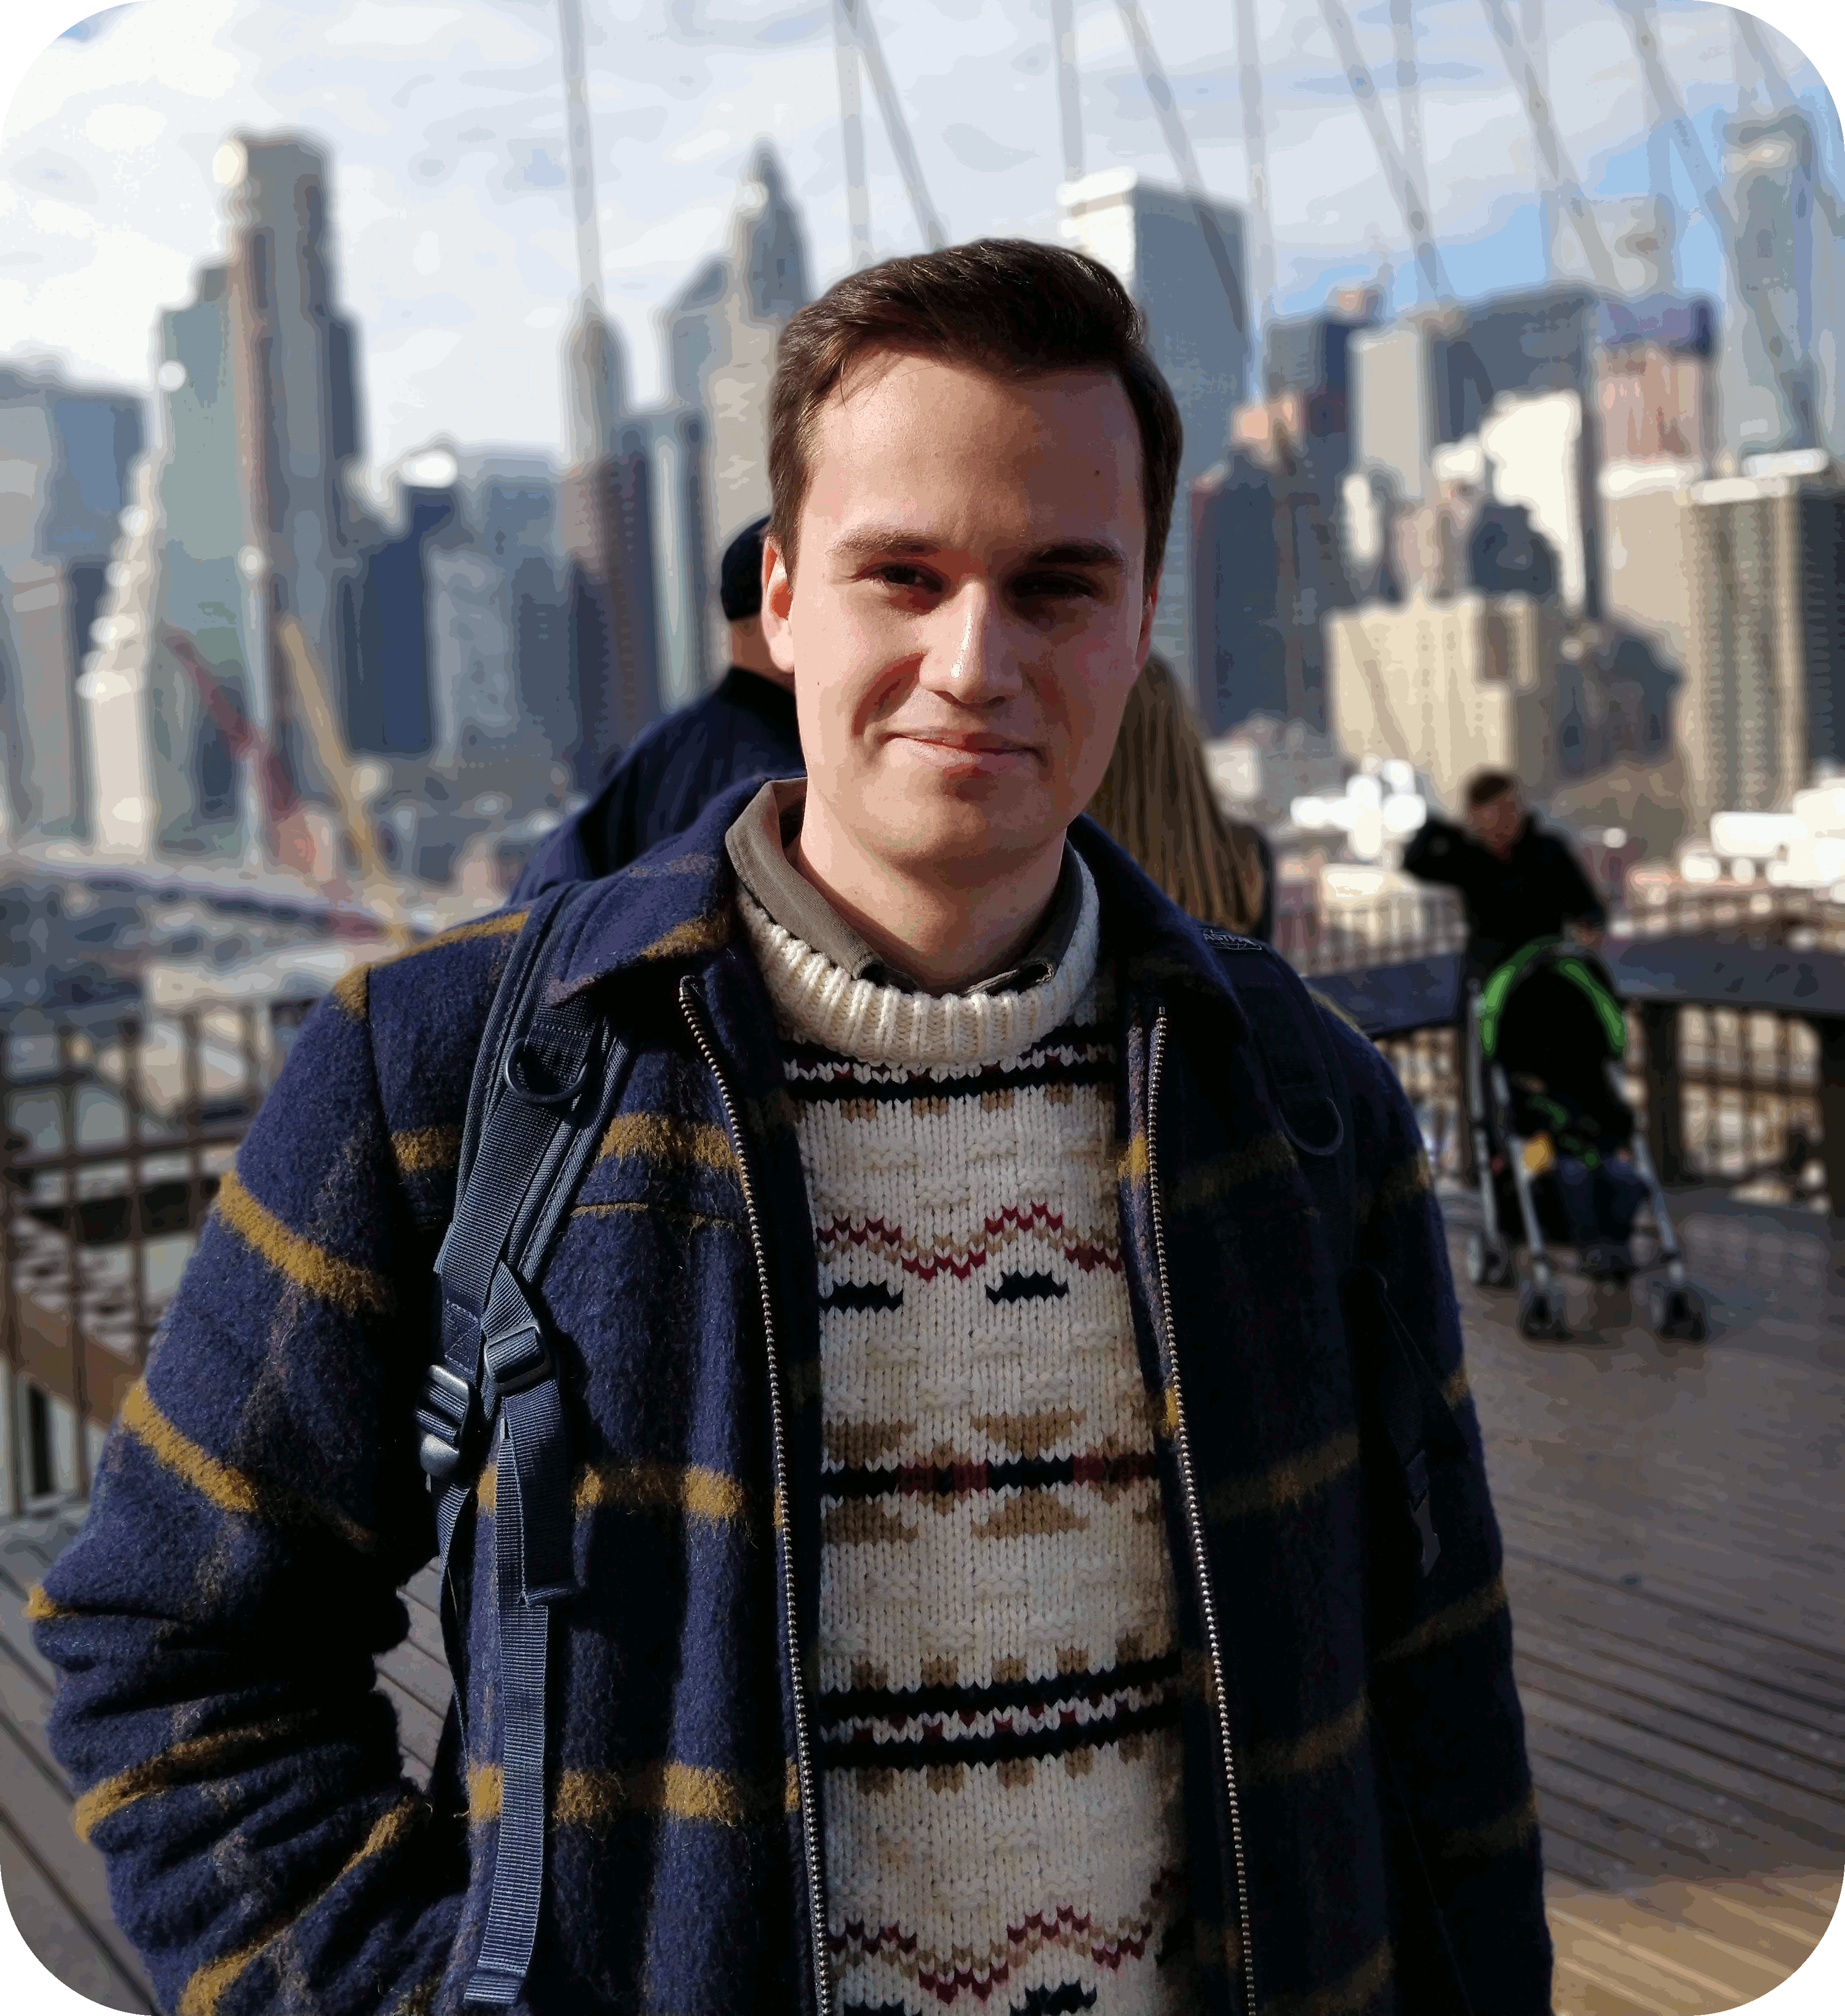
\includegraphics[width = 4cm]{Profile.png}
    \end{figure}
    \name{Jan}{Stevens}
    \hspace{0.6cm}
    \begin{tabular}[c]{lr}
        \contactline{Birthdate}{16-04-1998}\\
        \contactline{Birthplace}{Nijmegen}\\
        \contactline{Nationality}{Dutch}
    \end{tabular}
    
    \section{About me}

    \color{dark}

    tional Physics, with specialisation in Theoretical Analysis of Soft-Matter Simulations.\\
    Other interests: Computer Science, Data Science and AI.\\
    
    \section{Contacts}

    \renewcommand{\arraystretch}{1.1}

    \begin{tabular}{rl}
        \contactline{Phone}{(+32) 491 04 16 20} \\
        \contactline{Email}{jan.stevens2@kuleuven.be} \\
        \contactline{Website}{\href{https://www.jstevens.be/}{jstevens.be}} \\
        \contactline{GitHub}{\href{https://github.com/biogen98}{@biogen98}} \\
        \contactline{LinkedIn}{\href{https://www.linkedin.com/in/jan-adriaan-stevens}{/in/jan-adriaan-stevens}}
    \end{tabular}


    \section{Skills}

    \skill{Mathematics}{4}

    \skill{Python}{4}
    
    \skill{Data analysis}{4}
    
    \skill{\TeX}{3.5}

    \skill{Linux}{3.5}
    
    \skill{R}{3}
    
    \skill{Git}{3}

\end{textblock}

% Main

\vspace{-25pt}  % Change this value to adjust the position of the right

\section{Education}
\block{Secondary School: Sint-Hubertus College Pelt}{Sciences and Mathematics | 2010 - 2016}{}

\hfill

\block{Bachelor: KU Leuven}
{B.Sc. Physics | minor: Mathematics | 2016  - 2019}
{
    Relevant Coursework: Statistical Mechanics, Introduction to Quantum Mechanics, Particle Physics;
}

\hfill

\block{Master: KU Leuven}
{M.Sc. Theoretical Physics | Research Option: A.I. | 2019 - current}
{
    Relevant Coursework: Computational Physics, Mathematical Physics, Physical Modelling of Complex Systems
}

\hfill

\section{Courses \& Certificates}

\block{Peer Assisted Learning Tutor}{Course: Introduction to Quantum Mechanics | Spring semester 2019}{}

\hfill

\section{Extracurricular}

\block{Student representative KU Leuven}{member from 2017 - current}{
    Student representative for Physics students. \\
    Member of following committees:
    \vspace{1mm}
    \begin{itemize}
        \item Permanent Education Committee Physics
        \item Umbrella Education Council for Sciences
        \item Student Council KU Leuven
    \end{itemize}
}

\hfill

\block{Volunteer at St-Oda}{Summer camp 2015 | St-Odafeesten 2015}{
    Sint Oda is a service centre for children and adults with multiple physical and mental disabilities. As students we supported the staff.
}

\hfill

\section{Awards}
\ralewaysb Second Price \raleway "junior olympiade natuurwetenschappen" | May 2014

\hfill

\section{Languages}
\begin{itemize}
    \item \textbf{Dutch}: Native Language   
    \item \textbf{English}:  Full Professional Proficiency
    \item \textbf{French}: Professional Working Proficiency
    \item \textbf{German}: Limited Working Proficiency
\end{itemize}

\hfill

\section{Hobbies}
\begin{itemize}
    \item Walking my dog
    \item Literature
    \item Philosophy
\end{itemize}
\end{document}
